\normaltrue \difficilefalse \tdifficilefalse
\correctionfalse
%\UPSTIidClasse{11} % 11 sup, 12 spé
%\newcommand{\UPSTIidClasse}{11}

\exer{Exercice d'application $\star$ \label{PERF:02:C2:03:stab:64}}
%% CCP MP 2007
\setcounter{question}{0}\marginnote{\xpComp{PERF}{02}}%\index{Compétence C2-03}\index{Compétence PERF-02}
\index{Compétence C2-03}
\index{Schéma-blocs}
\index{Stabilite}

\ifcorrection
\else
\marginnote{\textbf{Pas de corrigé pour cet exercice.}}
\fi


\ifprof
\else
L'asservissement est donné par le schéma-blocs suivant. $H_{\text{BO}}(p) = \dfrac{4}{p\left( p+3,6\right)}$.  Le retard du système est de \SI{0,2}{s}.
De plus, $C(p)=K_c\dfrac{1+T_c p}{T_c p}$

\begin{marginfigure}
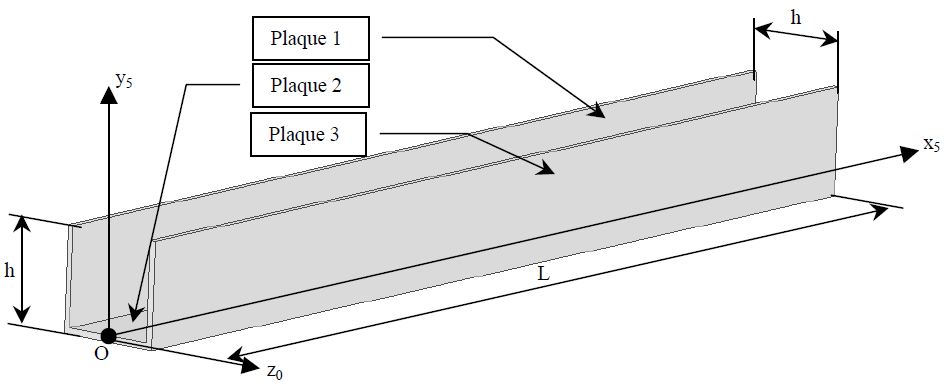
\includegraphics[width=\linewidth]{64_01}
\end{marginfigure}

\fi
 
\question{Tracer le diagramme de Bode asymptotique de $H_{\text{BO}}(p)$ pour des pulsations comprises entre \SI{0,5}{rad.s^{-1}} et \SI{50}{rad.s^{-1}}.}
\ifprof
\else 
\fi

\question{Tracer le diagramme de Bode du retard pour des pulsations comprises entre \SI{0,5}{rad.s^{-1}} et \SI{50}{rad.s^{-1}}.}
\ifprof
\else 
\fi


\ifprof
\else
On donne le diagramme de la FTBO retardée. 

\begin{marginfigure}
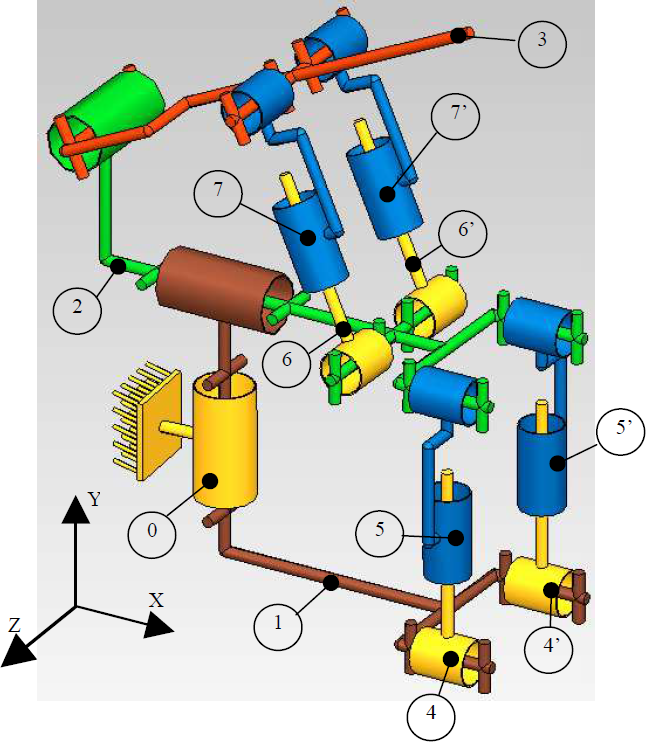
\includegraphics[width=\linewidth]{64_02}
\end{marginfigure}
\fi

\question{Déterminer le gain $K_c$ qui donne une marge de phase de 50\degres.}
\ifprof
\else 
\fi

\question{La constante $T_c$ qui laisse subsister une marge de phase d’environ 45\degres.}
\ifprof
\else 
\fi


\question{Quelle est l’erreur de traînage du système corrigé pour l’entrée en rampe considérée (en négligeant le retard).}
\ifprof
\else 
\fi


\ifprof
\else



\marginnote{Corrigé voir \ref{PERF:02:C2:03:stab:64}.}

\fi